\documentclass[tikz,preview]{standalone}
\usepackage{pgfplots}
\usetikzlibrary{arrows.meta}
\pgfplotsset{compat=newest, width=10cm, height=6cm}
\begin{document}
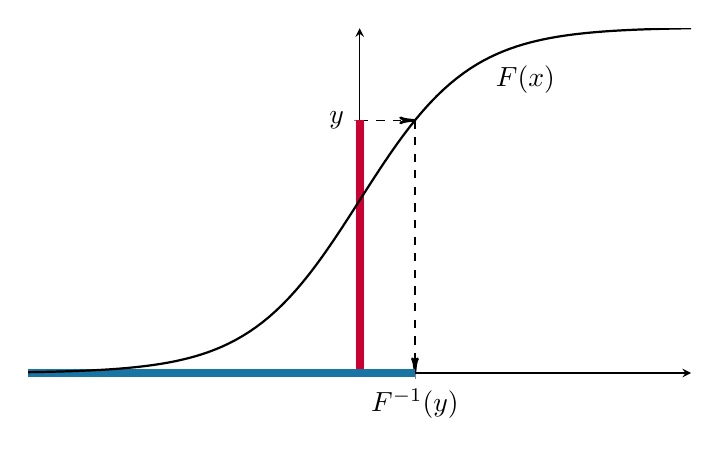
\begin{tikzpicture}

\begin{axis}[
    ymin=-0.009,
    axis x line = center,
    axis y line = center,
    xlabel = $$,
    ylabel = $$,
    xtick={1},
    xticklabels={$F^{-1}(y)$},
    ytick={0.731},
    yticklabels={$y$}
]
%Below the red parabola is defined


\addplot [dashed, arrows={->[line
width=1pt,black,length=2mm,width=1mm]}] (0,0.731) -- (1,0.731); -- 
(1,0) ;
\addplot [dashed, arrows={->[line
width=1pt,black,length=2mm,width=1mm]}]  (1,0.731) -- (1,0) ;

\addplot [draw=red!80!blue, line width=1mm] (0,0.0) -- (0,0.731);
\addplot [draw=blue!60!green!90, line width=1mm] (-6,0.0)--(1,0.0);
\addplot [
    domain=-6:6, 
    samples=100, 
    thick,
]
{1/(1+exp(-x))};

\node at (3,0.85) {$F(x)$};

\end{axis}
\end{tikzpicture}
\end{document}